% Created 2012-12-13 Thu 22:20
\documentclass[10pt, conference]{IEEEtran}
\usepackage[utf8]{inputenc}
\usepackage[T1]{fontenc}
\usepackage{fixltx2e}
\usepackage{graphicx}
\usepackage{longtable}
\usepackage{float}
\usepackage{wrapfig}
\usepackage{soul}
\usepackage{textcomp}
\usepackage{marvosym}
\usepackage{wasysym}
\usepackage{latexsym}
\usepackage{amssymb}
\usepackage{hyperref}
\tolerance=1000
\usepackage{balance}
\usepackage[numbers]{natbib}
\usepackage{graphicx}
\usepackage{dsfont}
\usepackage{mathtools}
\usepackage{amsmath}
\usepackage{subfigure}
\usepackage{multirow} %For tables
\usepackage{pdflscape}
\usepackage{rotating}
\usepackage{tabularx}
\usepackage{amsfonts}
\usepackage{booktabs}
\usepackage[amssymb]{SIunits}
\usepackage{fancyhdr}
\usepackage[format=hang,font=small,labelfont=bf]{caption}
\usepackage{hyperref}
\newcount\colveccount
\newcommand*\colvec[1]{\global\colveccount#1 \begin{bmatrix} \colvecnext }
\def\colvecnext#1{ #1 \global\advance\colveccount-1 \ifnum\colveccount>0 \expandafter\colvecnext \else \end{bmatrix}^{\top}\fi}
\providecommand{\alert}[1]{\textbf{#1}}

\title{Constrained Tool Planning in Work Space Using Inverse Jacobian Control}
\author{Adam Cantor, Jonathan Martin, Leo Keselman, Stewart Butler}
\date{2012-12-10 Mon}
\hypersetup{
  pdfkeywords={},
  pdfsubject={},
  pdfcreator={Emacs Org-mode version 7.8.11}}

\begin{document}

\maketitle






\begin{abstract}
This report details an approach to known object interaction with a
Schunk Arm. A motion planning theorem is applied with a focus on
workspace control. The implementation of this system was done in the
GRIP/DART simulation environment designed/used by the Golems Lab at
Georgia Tech.
\end{abstract}

\section{Introduction}
\label{sec-1}

  The purpose of this work is to create a methodology for interacting
  with known objects in a loosely defined workspace. This goal is
  directly in line with the DARPA robotics challenge to apply humanoid
  robots to search and rescue applications by using tools and
  exploration algorithms.

  No single robot can be equipped to deal with all environments equally
  well. A general purpose robot, given a concrete goal for which it is
  not configured correctly, must be able to use objects from its
  environment to reach its goals. In an anthropocentric environment this
  means that correctly wielding tools designed for human use gives a
  robot a degree of operational flexibility that would be otherwise
  impossible.


\begin{figure}[htb]
\centering
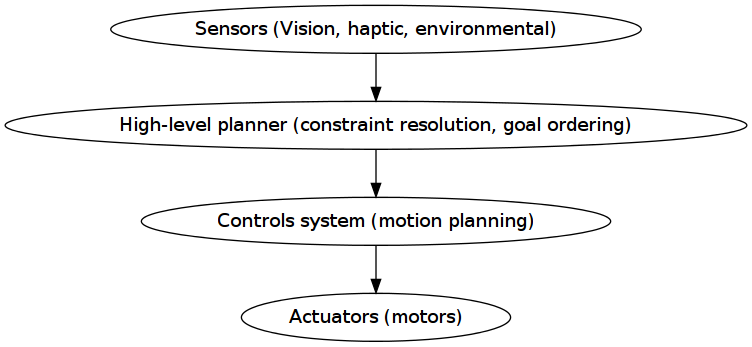
\includegraphics[width=8cm]{robot_layer_model_04acea6317138ac7fb5e808de063a70455ba7e53.png}
\caption{\label{fig:layer_model}Layer model of robot control systems.}
\end{figure}


  Using human-configured tools requires multiple layers of control and
  planning, as shown in figure \ref{fig:layer_model}.

\begin{enumerate}
\item Sensors - The robot must be capable of discerning its environment,
     discovering what constraints that environment will impose upon it,
     and constructing sub-goals in order to accomplish its target
     task. In an un-augmented anthropocentric environment, this means
     having a sufficiently sophisticated computer vision system (visual,
     radar, lidar, etc) to map the environment, recognize objects in the
     environment, and classify them as a given tool. It also means using
     haptic feedback (if possible) and torque feedback from the
     actuators during manipulation tasks as part of a control loop to
     ensure that the manipulated objects are behaving according to
     plan.
\item Planner - The robot needs a high level planner in order to take a
     goal state, break it into sub goals, match those sub goals with
     tasks it is able to handle, resolve any dependency conflicts, and
     order those goals into as efficient a plan as possible.
\item The control system is responsible for implementing each of the
     tasks necessary to accomplish a given sub-goal. This involves
     things like the lower-level motion planning necessary for
     manipulation, including workspace control.
\item Actuators - The robot must be capable of using its actuators to
     accomplish commands sent to them from the control
     system. Physically, one must be able to manipulate the tool in
     question. General purpose manipulators are not generally well
     suited for using tools designed for humanoid hands, and most
     commonly available humanoid hands have issues with grip strength,
     digit control, haptic sensing, and friction.
\end{enumerate}

  This document describes an effort to explore the challenges associated
  with general purpose tool usage from within a simulated
  environment. To reduce the scope of an otherwise unmanageable problem,
  the goal was simplified to be the control system for a single
  simulated Schunk LWA-4 arm, a 7-degree-of-freedom arm with an
  attachable manipulator. A screwdriver was chosen as the target tool,
  since it is the simplest tool that could be easily manipulated by a
  Schunk arm and still require a complex set of actions. In order to
  remove the necessity for a complicated sensor system, the work was
  done using the GRIP/DART simulation environment used by the Humanoid
  Robotics laboratory at Georgia Tech.

  Complications arose during the work which prevented all our goals from
  being reached. The implementation of the vital control elements of the
  proposed system was unusable due to bugs in the implemented workspace
  control. These were fixed to a usable point, but there was not enough
  time remaining to integrate the high level planner into the decision
  loop. As such, the robot is capable of all the physical manipulation
  tasks needed to reach its goal state, but those states must be
  manually traversed by a human in order for the simulation to
  work. These issues will be further discussed in later sections.
\section{Related Work}
\label{sec-2}

  Tool manipulation in workspace is very common in both research and
  industry. However, most of this tool manipulation is with specialized
  tools that are not designed for human manipulation, and the robots are
  generally used in environments where the state space is largely
  deterministic -- the planner for the robot can safely assume that a
  part will enter the assembly line at a certain time, reach a certain
  location in a certain orientation, and if there are any deviations
  from this expected behavior it will simply stop and alert a human of a
  problem.

  What made our planned approach unique is that we account both for the
  motion planning for the robot as well as the constraints of the
  tool. For example, when driving the screw into the target block, we
  must follow the screw with the driver (held in the manipulator) as it
  threads into the target block by matching `downward' translation with
  the rotation of the screw driver, then back the tool out and repeat
  until the screw is settled into the block. It also took into account
  the set of actions required to set up the environment -- finding the
  screw, placing it in the correct location for tool use, finding the
  tool, and finally driving the screw into the target block.

  Our chosen method of control is Resolved Rate Trajectory Planning,
  also known as pseudo-inverse Jacobian control. The principles behind
  Resolved Rate Trajectory Planning are well known in controls
  circles. The theory behind the implementation is not extremely
  complicated, making it an ideal method for workspace control of
  high-dimensional robots.\cite{survey_ik} The fact that it is a
  trajectory-following techinque makes it critical to our work, since we
  do not wish for the robot to deviate from our desired trajectory for
  risk of collision with the workpiece or losing control of the tool.

  Paul reviewed kinematic equations for simple manipulators like the one
  used here and explained how to determine the Jacobian for these
  manipulators.\cite{paul} Whitney investigated resolved rate trajectory
  planning and applied it to control manipulators under task
  constraints.\cite{whitney} Cheah described how Approximate Inverse
  Jacobian control could be used in dynamic environments to provide
  workspace control.\cite{cheah}
\section{Methods}
\label{sec-3}
\subsection{Simulation Software}
\label{sec-3-1}

   This project used the DART/GRIP visualization system developed by the
   Golems lab at the Georgia Tech center for Research in Intelligent
   Machines. It is especially developed for testing algorithms on rigid
   body manipulators. Although the work was meant to be used on a mobile
   robot, it is reasonable to assume that in the tool use domain, the
   mobile manipulator would be stationary and the work would be done by
   a 7 DOF arm.

   In DART/GRIP, the world is made up of objects and robots. Aside from
   a model, each object is described by its x,y, and z coordinate and
   made of links and revolute joints. The angle of each joint can be
   its rotation about the x,y, and z axis (roll, pitch, yaw). Robots are
   modified in the world inspector, and the change would automatically
   be reflected on the configurations of all the following links.

   This visualization software was chosen because it was optimized for
   manipulator motion, because it was already somewhat familiar to the
   research team and also because its source code was available in case
   any changes needed to be made. It is also open source and available
   to anyone wishing to replicate the results discussed here.
\subsection{Objects}
\label{sec-3-2}

   The manipulator for this project was the Schunk 7 degree of freedom
   arm with a hand. Although this is strictly a standalone manipulator,
   it simulated the 7 degrees of freedom and the hand on a potential
   mobile robot’s arm. The manipulator is shown in Figure \ref{fig:manipulator}.

   \begin{figure}[htb]
   \centering
   \includegraphics[width=8cm]{./img/Manipulator.jpg}
   \caption{\label{fig:manipulator}Manipulator model}
   \end{figure}

   The block, screw, and screwdriver were developed in Solidworks and
   imported into the world. These are shown in one particular
   configuration in Figure \ref{fig:objects}.

   \begin{figure}[htb]
   \centering
   \includegraphics[width=8cm]{./img/Objects.jpg}
   \caption{\label{fig:objects}Image capture of simulated environment, with objects.}
   \end{figure}
\subsection{High Level Planning}
\label{sec-3-3}

   The high level plan for screwing in a bolt is designed as follows:

\begin{enumerate}
\item Locate screw - Align the “palm” of the manipulator with the top of
      the head, such that the plane of palm is parallel to the plane of
      the bolt head. In our case, the palm had to be slightly above the
      screw to be able to grasp it. Of course this offset, if necessary,
      will be dictated by the particular application. (See Figure
      \ref{fig:screw})
\item Grasp the screw - Once the end effector and the bolt are aligned,
      close the fingers until they touch the screw. In a physical
      application, one would close the fingers until some force sensor
      on the fingers returns a certain value. In our case, we simply
      closed the fingers until a collision was detected. Collision
      detection was provided by DART/GRIP.
      \begin{figure}[htb]
      \centering
      \includegraphics[width=8cm]{./img/Picking_Up_Bolt.jpg}
      \caption{\label{fig:screw}Arm locating the screw object.}
      \end{figure}
\item Locate the goal - Once the end effector grasps the screw, move
      both to the goal configuration. In our case, this was the hole in
      the block.
      \begin{figure}[htb]
      \centering
      \includegraphics[width=8cm]{./img/Found_Block.jpg}
      \caption{\label{fig:block}Arm locating the block.}
      \end{figure}
\item Start screwing the bolt - Just use the arm to screw in the bolt
      initially so that it stays in place while the screwdriver is
      retrieved. (See Figure \ref{fig:driver})
\item Release the bolt - Leave it inside the whole, stationary.
\item Locate the screwdriver - Align the plam of the manipulator with the base of the screwdriver with an offset.
\item Grasp the screwdriver
      \begin{figure}[htb]
      \centering
      \includegraphics[width=8cm]{./img/Picked_Up_Driver.jpg}
      \caption{\label{fig:driver}Arm wielding the screw driver.}
      \end{figure}
\item Align screwdriver tip with bolt head - Here, there should be no
      offset between the tip and the bolt head. In a physical
      application, a force sensor on the hand could be used to determine
      when the screwdriver tip is making firm contact with the bolt
      head. In our case, we aligned the screwdriver and the bolt, then
      moved it closer until a collision was detected.
\item Screw in the bolt.
\end{enumerate}
\subsection{Low Level (Motion) Planning}
\label{sec-3-4}
\subsubsection{Resolved Rate Trajectory Planning}
\label{sec-3-4-1}

    Resolved rate trajectory planning, or pseudo-inverse Jacobian
    control, was used to move the manipulator from a current world
    configuration \( \mathbf{x_i} =
    \colvec{6}{x_i}{y_i}{z_i}{R_i}{P_i}{Y_i} \) to a target goal
    configuration \( \mathbf{x_f} =
    \colvec{6}{x_f}{y_f}{z_f}{R_f}{P_f}{Y_f}\) in a linear fashion. The
    world coordinates are described as \( 6 \times 1 \) vectors of X,Y,
    and Z positions with corresponding Roll, Pitch and Yaw.

    Resolved rate trajectory control stems from
    \ref{ eq:rate_trajectory}, where \(\mathbf{V_e}(t)\) is the end
    effector velocity at time \(t\), \(\mathbf{\alpha}\) is the joint
    space position vector describing the current configuration of the
    robot, and \(\mathbf{\dot{\alpha}} \) is the joint space velocity
    vector.

    \begin{equation}
    \label{ eq:rate_trajectory}
    \mathbf{V_{e}}(t)\mathbf{ = J(\alpha)\dot{\alpha}}
    \end{equation}

    This can be rearranged into \ref{eq:rate_trajectory_inv}.

    \begin{equation}
    \label{eq:rate_trajectory_inv}
    \mathbf{\dot{\alpha} = J(\alpha)^{-1}V_e(t)}.
    \end{equation}

    Thus, if the inverse Jacobian and desired end effector trajectory
    are known, it is possible to make a differential equation for the
    joint angles of the manipulator. In this case, the trajectory is to
    be linear, so \(\mathbf{V_e(t)}\) was a constant \(6 \times 1\) vector equal
    to \(\mathbf{x_f}-\mathbf{x_i}\).
\subsubsection{Extracting a target coordinate}
\label{sec-3-4-2}

    The world coordinate of a given node is generated from DART/GRIP as
    an affine transformation described by the \(4 \times 4\)
    homogeneous coordinate matrix \(C = \begin{bmatrix}
    \multicolumn{3}{c}{\mathbf{R}} & \mathbf{X_{xyz}} \\ 0 & 0 & 0 & 1 \end{bmatrix}\),
    so the \(6 \times 1\) XYZRPY vector representation must first be
    extracted.

    \(\mathbf{X_{xyz}}\) is a \(3 \times 1\) vector describing a point in
    3-space, and does not require any manipulation. \(\mathbf{R}\) is a \(3
    \times 3\) rotation matrix, so we convert this to roll-pitch-yaw as
    shown in equation \ref{eq:rpy}:

    \begin{equation}
    \label{eq:rpy}
    \mathbf{X_{rpy}} = \begin{bmatrix} \tan^{-1}(\frac{R_{2,1}}{R_{2,2}}) \\
    -\sin^{-1}(R_{2,0}) \\ \tan^{-1}(\frac{R_{1,0}}{R_{0,0}}) \end{bmatrix},
    \end{equation}

    This yields our target coordinates \(\mathbf{x_{f}}
    = \begin{bmatrix}X_{xyz} \\ X_{rpy} \end{bmatrix} \).
\subsubsection{Inverting the Jacobian}
\label{sec-3-4-3}

    A direct inverse of the Jacobian is not possible in our case, as
    our manipulator had 7 degrees of freedom producing a \(7 \times 6\)
    matrix. Instead, a Moore-Penrose pseudo-inverse was calculated
    according to equation \ref{eq:pseudoinv}.

    \begin{equation}
    \label{eq:pseudoinv}
    J(\alpha)^{\dagger} = J(\alpha)^{\top}(J(\alpha)J(\alpha)^{\top})^{-1}
    \end{equation}

    From this we compute for each time step the change in joint angles
    via equation \ref{eq:velocity}:

    \begin{equation}
    \label{eq:velocity}
    \dot{\alpha} = J(\alpha)^{\dagger}V_e(t)
    \end{equation}

    This is added to the previous time step's joint configuration and
    the robot is updated. The process continues until the global
    coordinates (both rotation and translation) of the end effector
    of the manipulator is less than a threshold distance $\epsilon$
    of the desired position. In other words,

    \begin{equation}
    \label{eq:distance}
    \| \mathbf{x_f - x_i} \| < \epsilon
    \end{equation}
\subsubsection{Joint limit avoidance}
\label{sec-3-4-4}

    This equation for the joint velocities is not always well
    behaved. In order to improve the results, we will use a variation
    of the joint-limits avoidance strategy described in
    \cite{luc_baron}.

    We now know from \ref{eq:velocity} the regular form of our
    velocity equation used to generate a trajectory toward our primary
    task. We will now augment that with an additional secondary task
    that will bias the trajectory towards keeping the joints as close
    to their zero points as possible.

    First, we augment equation \ref{eq:velocity}, so our equation
    describing the change in joint angles is now \ref{eq:vel_jl}.

    \begin{equation}
    \label{eq:vel_jl}
    \mathbf{\dot{\alpha} = J(\alpha)^{\dagger}V_e(t) + (1 -
    J(\alpha)^{\dagger}J(\alpha))h}
    \end{equation}

    The vector \(h\) is our secondary task, multiplied by \(\mathbf{
    (1 - J(\alpha)^{\dagger}J(\alpha))}\), the orthogonal complement
    of J($\alpha$). The result is a projection of \(\mathbf{h}\) into
    the null space of \(\mathbf{J(\alpha)}\), a ``virtual motion'' which
    results in a bias toward the secondary objective.

    The secondary task is constructed as  \(\mathbf{h} = \nabla z\),
    where \(z\) is a fitness function described in \ref{eq:z}.

    \begin{equation}
    \label{eq:z}
    \mathbf{ z = \frac{1}{2}(\alpha - \bar{\alpha})^{\top}W(\alpha -
    \bar{\alpha})}
    \end{equation}

    The variable \(\mathbf{\bar{\alpha}}\) is the joint position vector
    describing the mid-joint position; in our case, this is an all-zero
    vector, as the entire arm is constructed from symmetrically
    revolute joints centered around zero.

    The matrix \( \mathbf{W} \) is a diagonal weight matrix describing
    the acceptable deviation from this zero point -- if it ;is desirable
    for a particular joint to have a greater latitude during movement
    than another, altering the corresponding row in the weight matrix
    will generate that effect. In our case, an identity matrix was
    used, as we only needed a general bias away from the joint limits.

    The effect is that \(\mathbf{h}\) describes a gradient where the
    zero positions on each joint is a minima, growing steeper as you
    progress further away from this center point. When projected into
    the null space of \(\mathbf{J_\alpha}\), it will cause joints that
    are otherwise unconstrained by the target motion to descend toward
    their zero positions, preventing the robot from approaching too
    close to the joint limits and preventing some of the anomalous
    behavior produced by unconstrained inverse Jacobian control.
\subsection{Object manipulation}
\label{sec-3-5}

   In the real world, the actual manipulation of an object is a trivial
   task -- once you grasp the object, it will behave as defined by the
   laws of physics, and can be treated as an extension of the end
   effector. However, the DART/GRIP simulation package does not
   currently support true connection of manipulated world objects as
   parts of the kinematic model of the robot, so the position of the
   world object must be manually updated according to the position of
   the end effector that is ``grasping'' it.

   Maintaining the relationship between the end effector and the grasped
   object is difficult using XYZ-RPY coordinates since any accidental
   change in the order of rotation will cause resulting transform to
   change. However, describing the different positions and orientations
   of the end effector and target object as the \(4 \times 4\) matrices
   of homogeneous coordinates describing the affine transformation used
   to take them from the global origin to their current global
   coordinates simplifies the task immensely.

   Instead of making multiple operations to transform the grasped object
   via relative rotations and translations from its previous position,
   we need now only describe the affine transformation \(\mathbf{R}\)
   which takes an object at coordinates \(\mathbf{O}\) to the end
   effector coordinates \(\mathbf{E}\), as calculated in equation
   \ref{eq:affinerel}.

   \begin{equation}\label{eq:affinerel}
   \mathbf{R} = \mathbf{E}^{-1}\mathbf{O}
   \end{equation}

   Subsequently, updating the position of object \(\mathbf{O}\) to
   \(\mathbf{O'}\) is a simple matrix multiplication of the new end
   effector location \(\mathbf{E'}\) by the relationship \(\mathbf{R}\),
   as shown in equation \ref{eq:affineup}.

   \begin{equation}\label{eq:affineup}
   \mathbf{O'} = \mathbf{E'}\mathbf{R}
   \end{equation}

   Setting the new location requires transforming the homogeneous
   coordinates back into global XYZ-RPY coordinates, as DART/GRIP do not
   currently expose a function for setting an objects position using
   homogeneous coordinates, but performing the transformations with
   homogeneous coordinates greatly reduces the risk of error.
\subsection{Task motion -- driving the screw}
\label{sec-3-6}

   Once the screw is in place, the screw driving motion is performed to
   keep it stationary at the block while the screwdriver is
   retrieved. The screw driving motion pattern consists of a rotation of
   the end effector about its axis by 60 degrees, a release event,
   anti-rotating the end effector 120 degrees (for a net -60 degrees
   away from the zero point), re-grasping, and repeating as necessary.

   A similar motion pattern is used when the screwdriver is in use,
   though with a significant offset to compensate for the longer
   tool. Though currently unimplemented, a second modification to the
   motion pattern when the tool is in use is a motion away from the tool
   during the anti-rotation rather than a release and re-grasp motion
   that leaves the tool suspended in midair.
\section{Experiments}
\label{sec-4}

  We were unable to perform any rigorous experimentation due to the
  broken inverse Jacobian workspace controller. However, during our
  attempts to debug the controller and lower motion planning, we did
  observe some extremely interesting behaviors in the failures produced
  by the inverse Jacobian controller producing bad output.

  The first problem we developed appeared after adding Roll, Pitch, and Yaw to
  the target coordinates. If the target coordinates was near the outside
  of the arm's range of motion, it would attempt to drive its joints
  past their theoretical limits -- opening up the inspection tab in GRIP
  showed occasional joint rotations in excess of \textpm{} 4000 degrees, and
  typical rotations of at least \textpm{} 200 on the primary joints. Figure \ref{fig:nojoints}
  \begin{figure}[htb]
  \centering
  \includegraphics[width=8cm]{./img/VideoGrab1.jpg}
  \caption{\label{fig:nojoints}Failure mode without joint limits}
  \end{figure}

  At first we believed this to be a result of the objects being placed
  outide of the end effector's range of motion, but when the orientation
  constraint was relaxed the controller would correctly find a solution
  in just the X,Y,Z axes. This is the point at which we relaxed the
  threshold for a correct solution, and our results improved
  significantly.

  However, after a more complicated set of motions the arm would
  occasionally contort itself into a configuration that caused it to
  detect the shortest path to the destination coordinate to take it
  through its joint limits. This resulted in similar behavior as the
  previous figure depicted, and was prevalent enough that it still
  prevented us from completing the entire manipulation
  procedure. Further research yielded the technique dicussed in section
  \ref{sec-3-4-4}. Implementation took quite a lot of further
  iteration, but when the necessary modifications had been made we
  activated the path finding routine again and found the arm contorting
  worse than before, as shown in figure \ref{fig:scaryjoints}. This
  behavior was caused by an inversion of the gradient values for the
  secondary objective, which effectively caused the arm to run as far
  away from its neutral joint position as possible.

  \begin{figure}[htb]
  \centering
  \includegraphics[width=8cm]{./img/VideoGrab2.jpg}
  \caption{\label{fig:scaryjoints}Failure mode with inverted gradient joint limits}
  \end{figure}

  After fixing this behavior, the workspace controller appears to work
  correctly, but no time remains for the implementation of the high
  level planner to permit further experimentation.
\section{Analysis}
\label{sec-5}
\subsection{Completeness}
\label{sec-5-1}

   The main underlying principle behind our motion planning was Resolved
   Rate Trajectory control, as described in section \ref{sec-3}.  This
   strategy can never be shown to be complete. It would not be able to
   find a goal if the start or end configuration was at a singularity. A
   singularity is any location in the workspace where the Jacobian loses
   rank. In this case, the pseudo-inverse becomes very large(inverse of
   a very small number). The algorithm then returns inaccurate joint
   velocities. This is really just a mathematical problem and is a
   shortcoming with the planning strategy. Singularities occur when
   joints are directly aligned and thus generally tend to happen near
   the boundaries of the workspace. Thus, Jacobian control can not be
   guaranteed to find a suitable plan if it exists.
\subsection{Optimality}
\label{sec-5-2}

   Jacobian control can be thought of as optimal in that sense that it
   follows the desired trajectory arbitrarily closely. It depends on how
   small of a time step is taken in integrating the differential
   equation for \(\mathbf{\dot{\alpha}}\). This again hinges on the
   start and end configurations not being singularities. In this case,
   the Inverse Jacobian method will not find a solution, much less an
   optimal one. However, if the start and end configuration are safely
   within the reachable workspace and a specific trajectory is
   necessary, this method can be very useful.
\subsection{Efficiency}
\label{sec-5-3}


   Jacobian control is quite efficient in time and space. In both of
   these parameters, complexity is linear to the length of the desired
   path. The most time and space consuming part is the inverse of the
   Jacobian. In our case, this always takes the same amount of time
   because the size of the Jacobian is always 6x7. For more degree of
   freedom arms, the Jacobian would have more columns, but never so
   many that the computation of the inverse becomes problematic.
\subsection{Summary}
\label{sec-5-4}


   Overall, the algorithms used were chosen for efficiency instead of
   optimality and completeness. In practice, true optimality is rarely
   a high priority — “second best” plans are usually good enough, often
   with a large enough gain in speed for real time applications. For
   our particular application, optimality was a low priority and thus
   the Jacobian method was deemed sufficient. It’s also worth noting
   that this method is relatively easy to implement compared to other
   algorithms accomplishing the same thing. No inverse kinematics are
   required and the only lengthy part as far as setup is the synthesis
   of the Jacobian.
\section{Discussion}
\label{sec-6}

   Driving a screw seemed like a reasonable task for a first experiment
   with constrained tool use with anthropocentric tools, since such a
   task is easy to decompose into a subset of simple goals. General tool
   planning is a hard problem with a very high computational complexity;
   by breaking down the problem into highly specialized subgoals, we
   drastically reduce the scope of the problem, but also make solutions
   inapplicable to other tool problems.

   Though we were quick to reduce scope away from the impossible
   problems, we were unable to correctly estimate the amount of time
   required to debug our workspace control system.  Without some form of
   control system, we were left unable to implement the higher level
   logic to get the desired task-planning behavior. After the
   demo/presentation, we were able to successfully integrate joint-limit
   avoidance into the Jacobian control system, which yielded proper
   low-level motion planning, but did not leave enough time to
   generalize the motion tasks and implement the high-level planner.

   The inverse kinematics needed to orient tools properly was much more
   complicated than we expected, especially in an application with such
   tight constraints on the final position and orientation of the end
   effector (aligning the screw into the hole correctly). RRTs were
   sufficient when a start and end \emph{jointspace} configuration is
   known to generate the desired workspace configuration, but no
   solution is possible when only the desired end effector position is
   known without some form of inverse kinematics.

   Our problems with the workspace control system started when we
   attempted to integrate the Roll, Pitch, and Yaw coordinates into the
   gradient descent behavior. Augmenting the linear Jacobian with the
   angular Jacobian (turning it from a \(3 \times \n \) matrix into a
   \(6 \times n \) matrix) was simple enough, but resulted in very
   bizarre behaviors. The initial problem was an unclear conversion
   between degrees and radians, but after that was fixed the behavior
   still resulted in the robot clipping through itself and the
   table. With further debugging we noticed that our distance
   calculation was causing the issues, as the threshold was not large
   enough to permit an acceptable offset in all six dimensions so the
   controller would thrash as it approached its solution. This improved
   performance, but did not solve the fundamental problem.

   We eventually narrowed down the underlying issue to the lack of joint
   limits. The motion planner would ignore the joint limits and, in
   searching for the correct joint-space configuration to reach its
   destination, would contort itself into impossible positions. After
   this was discovered, the joint-limit avoidance method described by
   Baron \cite{luc_baron} was implemented and behavior stabilized.

   At this point, the only remaining tasks are the integration of a
   high-level planner -- easily done by integrating FF or another domain
   planner into the current decision loop -- and working out the few
   remaining bugs in the coordinate system (offset from the tools,
   etc). Given an additional few days to a week, these changes could be
   easily integrated.

\bibliographystyle{plain}
\bibliography{rip_2012_final_project}

\clearpage
\newpage
\appendix
\section{Additional Questions}
\label{sec-7}
\subsection{How much time did your group spend on this project in total? How much of it has gone to making mistakes, experimenting, etc. as opposed to direct implementation? Reflect.}
\label{sec-7-1}

   We estimate we spent around 60 hours on this project. Much of the
   time was spent trying to understand the inner workings of
   DART/GRIP. There were a couple small bugs that took a lot of time to
   figure out. Another issue was that we didn’t quite realize the
   limitation of the inverse Jacobian approach and we spent a lot of
   time trying to figure out why the plans were misbehaving, when the
   whole time it was because of singularities. Another issue was
   understand how to extract RPY information of the end effector. We
   weren’t sure how the transform matrix was calculated so it was
   difficult to extract RPY from it.
\subsection{How much time do you think it would take to complete your initial goal?}
\label{sec-7-2}

   The initial goal was what we actually implemented plus a high level
   planner that would decide order of operations and so on. This would
   have involved putting the domain into PDDL, using one of the planners
   attempted earlier in the semester, and then integrating this with
   DART/GRIP. This is theoretically simple but the details may have
   taken another 40 hours or so.
\subsection{Given what you have completed and comparing your work with other groups', what grade do you think you should receive?}
\label{sec-7-3}

   Some groups had significantly more impressive results, but this may
   have been partially aided by their own work previously done for
   another objective. Overall, we think we deserve around a B.

\end{document}
